\documentclass[11pt,a4paper]{report}
\usepackage[textwidth=37em,vmargin=30mm]{geometry}
\usepackage{calc,xunicode,amsmath,amssymb,paralist,enumitem,tabu,booktabs,datetime2,xeCJK,xeCJKfntef,listings}
\usepackage{tocloft,fancyhdr,tcolorbox,xcolor,graphicx,eso-pic,xltxtra,xelatexemoji}

\newcommand{\envyear}[0]{2025}
\newcommand{\envdatestr}[0]{2025-10-05}
\newcommand{\envfinaldir}[0]{webdb/2025/20251005/final}

\usepackage[hidelinks]{hyperref}
\hypersetup{
    colorlinks=false,
    pdfpagemode=FullScreen,
    pdftitle={Web Digest - \envdatestr}
}

\setlength{\cftbeforechapskip}{10pt}
\renewcommand{\cftchapfont}{\rmfamily\bfseries\large\raggedright}
\setlength{\cftbeforesecskip}{2pt}
\renewcommand{\cftsecfont}{\sffamily\small\raggedright}

\setdefaultleftmargin{2em}{2em}{1em}{1em}{1em}{1em}

\usepackage{xeCJK,xeCJKfntef}
\xeCJKsetup{PunctStyle=plain,RubberPunctSkip=false,CJKglue=\strut\hskip 0pt plus 0.1em minus 0.05em,CJKecglue=\strut\hskip 0.22em plus 0.2em}
\XeTeXlinebreaklocale "zh"
\XeTeXlinebreakskip = 0pt


\setmainfont{Brygada 1918}
\setromanfont{Brygada 1918}
\setsansfont{IBM Plex Sans}
\setmonofont{JetBrains Mono NL}
\setCJKmainfont{Noto Serif CJK SC}
\setCJKromanfont{Noto Serif CJK SC}
\setCJKsansfont{Noto Sans CJK SC}
\setCJKmonofont{Noto Sans CJK SC}

\setlength{\parindent}{0pt}
\setlength{\parskip}{8pt}
\linespread{1.15}

\lstset{
	basicstyle=\ttfamily\footnotesize,
	numbersep=5pt,
	backgroundcolor=\color{black!5},
	showspaces=false,
	showstringspaces=false,
	showtabs=false,
	tabsize=2,
	captionpos=b,
	breaklines=true,
	breakatwhitespace=true,
	breakautoindent=true,
	linewidth=\textwidth
}






\newcommand{\coverpic}[2]{
    % argv: itemurl, authorname
    Cover photo by #2~~(\href{#1}{#1})
}
\newcommand{\makeheader}[0]{
    \begin{titlepage}
        % \newgeometry{hmargin=15mm,tmargin=21mm,bmargin=12mm}
        \begin{center}
            
            \rmfamily\scshape
            \fontspec{BaskervilleF}
            \fontspec{Old Standard}
            \fontsize{59pt}{70pt}\selectfont
            WEB\hfill DIGEST
            
            \vfill
            % \vskip 30pt
            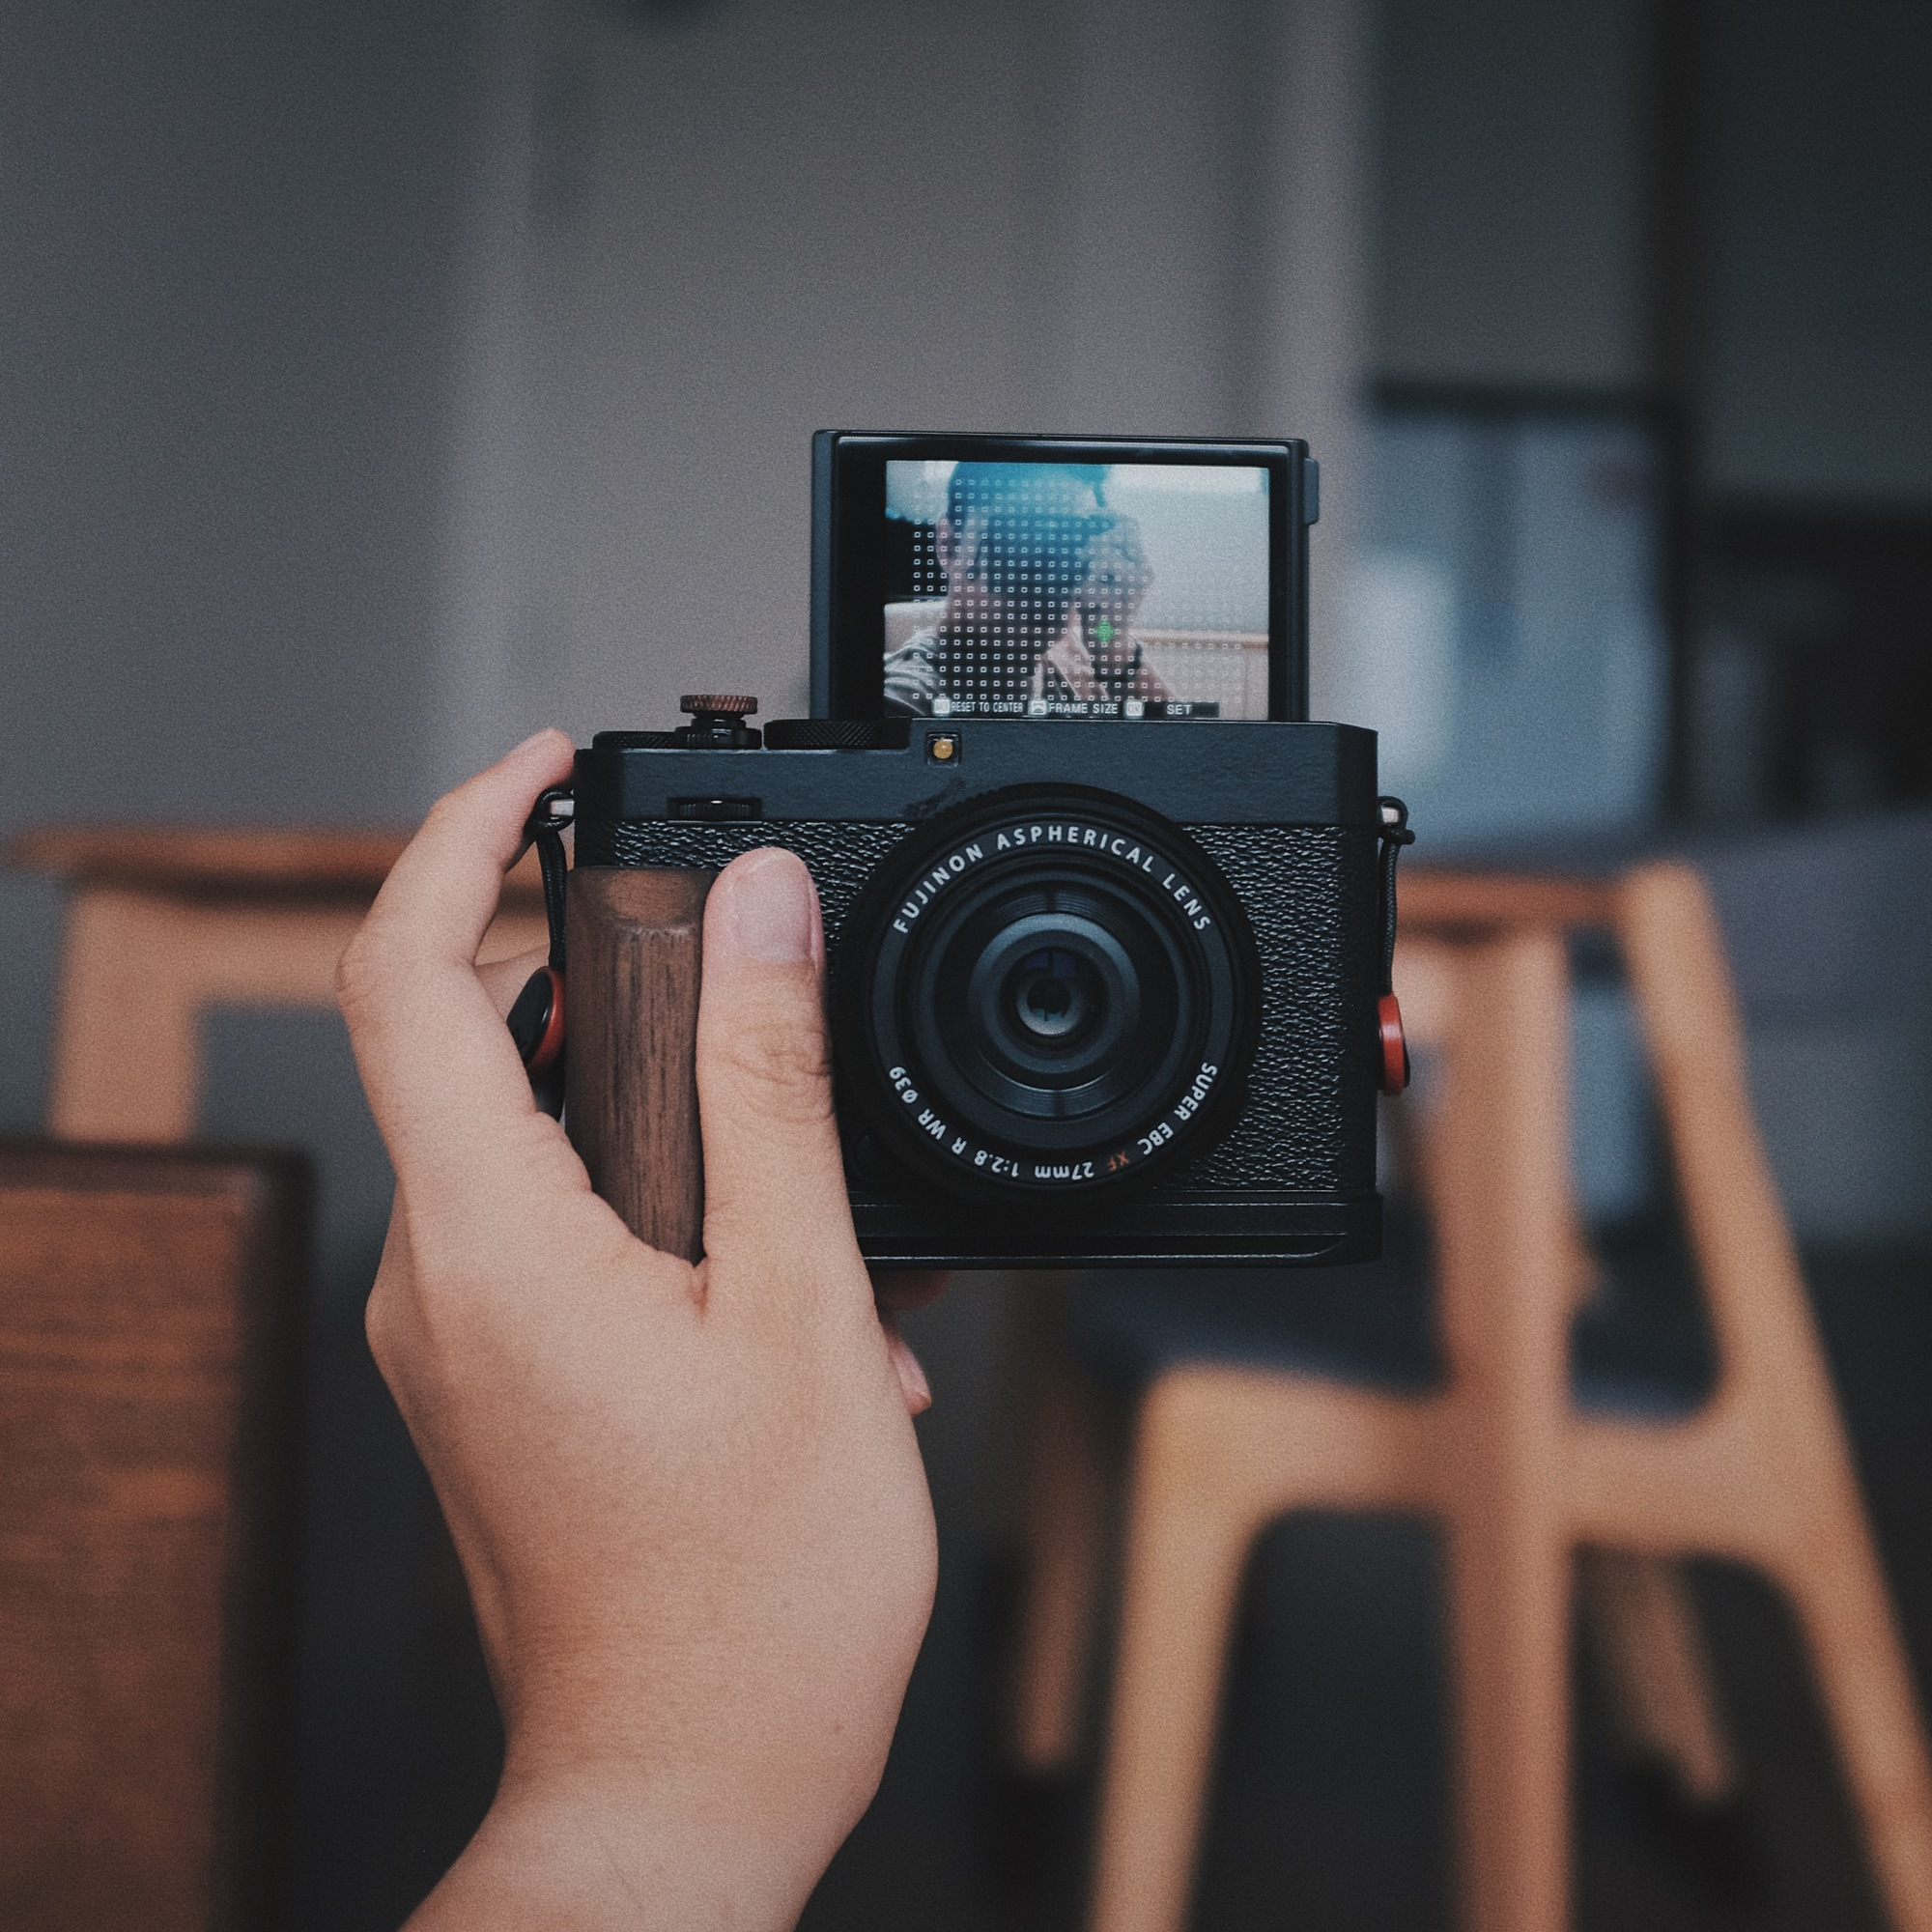
\includegraphics[width=\linewidth]{\envfinaldir/coverpic-prod.jpg}\par
            % \vskip 30pt
            \vfill

            \normalsize\rmfamily\scshape
            \copyright{} The Web Digest Project \hfill\large \envdatestr
        \end{center}
    \end{titlepage}
    % \restoregeometry
}
\newcommand{\simplehref}[1]{%
    \textcolor{blue!80!green}{\href{#1}{#1}}%
}
\renewcommand{\contentsname}{\center\Huge\sffamily\bfseries Contents\par\vskip 20pt}
\newcounter{ipartcounter}
\setcounter{ipartcounter}{0}
\newcommand{\ipart}[1]{
    % \vskip 20pt
    \clearpage
    \stepcounter{ipartcounter}
    \phantomsection
    \addcontentsline{toc}{chapter}{#1}
    % \begin{center}
    %     \Huge
    %     \sffamily\bfseries
    %     #1
    % \end{center}
    % \vskip 20pt plus 7pt
}
\newcounter{ichaptercounter}
\setcounter{ichaptercounter}{0}
\newcommand{\ichapter}[1]{
    % \vskip 20pt
    \clearpage
    \stepcounter{ichaptercounter}
    \phantomsection
    \addcontentsline{toc}{section}{\numberline{\arabic{ichaptercounter}}#1}
    \begin{center}
        \Huge
        \sffamily\bfseries
        #1
    \end{center}
    \vskip 20pt plus 7pt
}
\newcommand{\entrytitlefont}[1]{\subsection*{\raggedright\Large\sffamily\bfseries#1}}
\newcommand{\entryitemGeneric}[2]{
    % argv: title, url
    \parbox{\linewidth}{
        \entrytitlefont{#1}\par\vskip 5pt
        \footnotesize\ttfamily\mdseries
        \simplehref{#2}
    }\vskip 11pt plus 11pt minus 1pt
}
\newcommand{\entryitemGithub}[3]{
    % argv: title, url, desc
    \parbox{\linewidth}{
        \entrytitlefont{#1}\par\vskip 5pt
        \footnotesize\ttfamily\mdseries
        \simplehref{#2}\par\vskip 5pt
        \small\rmfamily\mdseries#3
    }\vskip 11pt plus 11pt minus 1pt
}
\newcommand{\entryitemAp}[3]{
    % argv: title, url, desc
    \parbox{\linewidth}{
        \entrytitlefont{#1}\par\vskip 5pt
        \footnotesize\ttfamily\mdseries
        \simplehref{#2}\par\vskip 5pt
        \small\rmfamily\mdseries#3
    }\vskip 11pt plus 11pt minus 1pt
}
\newcommand{\entryitemHackernews}[3]{
    % argv: title, hnurl, rawurl
    % \parbox{\linewidth}{
    %     \entrytitlefont{#1}\par\vskip 5pt
    %     \footnotesize\ttfamily\mdseries
    %     \simplehref{#3}\par
    %     \textcolor{black!50}{\href{#2}{#2}}
    % }\vskip 11pt plus 11pt minus 1pt
    \begin{minipage}{\linewidth}
            \entrytitlefont{#1}\par\vskip 5pt
            \footnotesize\ttfamily\mdseries
            \simplehref{#3}\par
            \textcolor{black!50}{\href{#2}{#2}}
    \end{minipage}\par\vskip 11pt plus 11pt minus 1pt
}







\begin{document}

\makeheader

\tableofcontents\clearpage




\ipart{Developers}
\ichapter{Hacker News}
\entryitemTwoLinks{The UK is still trying to backdoor encryption for Apple users}{https://news.ycombinator.com/item?id=45476273}{https://www.eff.org/deeplinks/2025/10/uk-still-trying-backdoor-encryption-apple-users}

\entryitemTwoLinks{ProofOfThought: LLM-based reasoning using Z3 theorem proving}{https://news.ycombinator.com/item?id=45475529}{https://github.com/DebarghaG/proofofthought}

\entryitemTwoLinks{Privacy Harm Is Harm}{https://news.ycombinator.com/item?id=45474441}{https://www.eff.org/deeplinks/2025/10/privacy-harm-harm}

\entryitemTwoLinks{A comparison of Ada and Rust, using solutions to the Advent of Code}{https://news.ycombinator.com/item?id=45473861}{https://github.com/johnperry-math/AoC2023/blob/master/More\_Detailed\_Comparison.md}

\entryitemTwoLinks{How I influence tech company politics as a staff software engineer}{https://news.ycombinator.com/item?id=45473852}{https://www.seangoedecke.com/how-to-influence-politics/}

\entryitemTwoLinks{Self-hosting email like it's 1984}{https://news.ycombinator.com/item?id=45473730}{https://maxadamski.com/blog/2025/10/email.html}

\entryitemTwoLinks{Flock's gunshot detection microphones will start listening for human voices}{https://news.ycombinator.com/item?id=45473698}{https://www.eff.org/deeplinks/2025/10/flocks-gunshot-detection-microphones-will-start-listening-human-voices}

\entryitemTwoLinks{Circular Financing: Does Nvidia's \$110B Bet Echo the Telecom Bubble?}{https://news.ycombinator.com/item?id=45473033}{https://tomtunguz.com/nvidia\_nortel\_vendor\_financing\_comparison/}

\entryitemTwoLinks{How functional programming shaped and twisted front end development}{https://news.ycombinator.com/item?id=45473019}{https://alfy.blog/2025/10/04/how-functional-programming-shaped-modern-frontend.html}

\entryitemTwoLinks{Google removes ICE-spotting app following Apple's ICEBlock crackdown}{https://news.ycombinator.com/item?id=45472799}{https://www.theverge.com/news/791533/google-apple-ice-tracking-app-store-red-dot-iceblock}

\entryitemTwoLinks{Thunderscan: A clever device transforms a printer into a scanner (2004)}{https://news.ycombinator.com/item?id=45472765}{https://www.folklore.org/Thunderscan.html}

\entryitemTwoLinks{The Buchstabenmuseum Berlin is closing}{https://news.ycombinator.com/item?id=45472678}{https://www.buchstabenmuseum.de/en/}

\entryitemTwoLinks{Scientists are discovering a powerful new way to prevent cancer}{https://news.ycombinator.com/item?id=45472614}{https://www.economist.com/science-and-technology/2025/09/02/scientists-are-discovering-a-powerful-new-way-to-prevent-cancer}

\entryitemTwoLinks{Paged Out Issue \#7 [pdf]}{https://news.ycombinator.com/item?id=45472319}{https://pagedout.institute/download/PagedOut\_007.pdf}

\entryitemTwoLinks{Alibaba cloud FPGA: the \$200 Kintex UltraScale+}{https://news.ycombinator.com/item?id=45471136}{https://essenceia.github.io/projects/alibaba\_cloud\_fpga/}

\entryitemTwoLinks{Toyota runs a car-hacking event to boost security (2024)}{https://news.ycombinator.com/item?id=45470206}{https://toyotatimes.jp/en/spotlights/1061.html}

\entryitemTwoLinks{New antibiotic targets IBD and AI predicted how it would work}{https://news.ycombinator.com/item?id=45469579}{https://healthsci.mcmaster.ca/new-antibiotic-targets-ibd-and-ai-predicted-how-it-would-work-before-scientists-could-prove-it/}

\entryitemTwoLinks{Track which Electron apps slow down macOS 26 Tahoe}{https://news.ycombinator.com/item?id=45469468}{https://avarayr.github.io/shamelectron/}

\entryitemTwoLinks{Sora Update \#1}{https://news.ycombinator.com/item?id=45469437}{https://blog.samaltman.com/sora-update-number-1}

\entryitemTwoLinks{Discord customer service data breach leaks user info and scanned photo IDs}{https://news.ycombinator.com/item?id=45469436}{https://www.theverge.com/news/792032/discord-customer-service-data-breach-hack}\ichapter{Phoronix}
\entryitemGeneric{\hskip 0pt{}Linux 6.18 Lands Intel FRED Update For Late Incompatible Change To Spec}{https://www.phoronix.com/news/Linux-6.18-Intel-FRED}

\entryitemGeneric{\hskip 0pt{}Many Debian/Ubuntu Packages For Intel Accelerators \& Other Intel Software Have Been Orphaned}{https://www.phoronix.com/news/Intel-Debian-Packages-Orphaned}

\entryitemGeneric{\hskip 0pt{}F2FS Lands Performance Improvements In Linux 6.18}{https://www.phoronix.com/news/Linux-6.18-F2FS}

\entryitemGeneric{\hskip 0pt{}Cairo-Dock 3.6 Released With Wayland Support \& HiDPI}{https://www.phoronix.com/news/Cairo-Dock-3.6-Released}

\entryitemGeneric{\hskip 0pt{}Linux 6.18 IOMMU Changes For Intel, AMD, Apple \& RISC-V}{https://www.phoronix.com/news/Linux-6.18-IOMMU}

\entryitemGeneric{\hskip 0pt{}ISD 0.6 Released For Interactive Systemd Management}{https://www.phoronix.com/news/interactive-systemd-isd-0.6}

\entryitemGeneric{\hskip 0pt{}SMB3 \& KSMBD See Performance Improvements With Linux 6.18}{https://www.phoronix.com/news/Linux-6.18-SMB3-KSMBD}

\entryitemGeneric{\hskip 0pt{}KDE Plasma 6.5 Sees More Fixes \& More Early Feature Work For Plasma 6.6}{https://www.phoronix.com/news/KDE-Plasma-6.5-Beta-2-Week-Fix}

\entryitemGeneric{\hskip 0pt{}DM-PCACHE Merged For Linux 6.18 Along With Other DeviceMapper Changes}{https://www.phoronix.com/news/Linux-6.18-DM}


\ipart{Developers~~~~(zh-Hans)}
\ichapter{Solidot}
\entryitemGeneric{\hskip 0pt{}英特尔与 AMD 磋商代工芯片}{https://www.solidot.org/story?sid=82471}

\entryitemGeneric{\hskip 0pt{}印度高等法院要求医生书写清晰的处方}{https://www.solidot.org/story?sid=82470}

\entryitemGeneric{\hskip 0pt{}黑客声称入侵了 Red Hat 的 GitHub 代码库}{https://www.solidot.org/story?sid=82469}

\entryitemGeneric{\hskip 0pt{}千禧一代癌症发病率在上升}{https://www.solidot.org/story?sid=82468}

\entryitemGeneric{\hskip 0pt{}城市空气检测出致病性酵母菌株}{https://www.solidot.org/story?sid=82467}

\entryitemGeneric{\hskip 0pt{}珍·古道尔去世,享年 91 岁}{https://www.solidot.org/story?sid=82466}\ichapter{V2EX}
\entryitemGeneric{\hskip 0pt{}[iOS] ios26 的 bug 么? sim 卡要重新解锁。}{https://www.v2ex.com/t/1163386}

\entryitemGeneric{\hskip 0pt{}[分享发现] 发现一个好用的 App: NewPipe,能够屏蔽 Youtube 的广告,还能后台播放和悬浮窗}{https://www.v2ex.com/t/1163385}

\entryitemGeneric{\hskip 0pt{}[剧集] 国庆无聊, 请推荐各种好看的短句/爽剧/动画等}{https://www.v2ex.com/t/1163384}

\entryitemGeneric{\hskip 0pt{}[分享创造] 写了个 Sora2 取无水印视频的工具}{https://www.v2ex.com/t/1163383}

\entryitemGeneric{\hskip 0pt{}[问与答] 灵异事件,手机半夜自动拨打电话}{https://www.v2ex.com/t/1163381}

\entryitemGeneric{\hskip 0pt{}[问与答] 我真不行了,来个 MOD 大佬解决我的问题吧,很简单的}{https://www.v2ex.com/t/1163380}

\entryitemGeneric{\hskip 0pt{}[分享发现] 今天在 windows11 上安装 claude code,记录一下安装过程}{https://www.v2ex.com/t/1163379}

\entryitemGeneric{\hskip 0pt{}[MacBook] 48+512 不是一个合理的配置}{https://www.v2ex.com/t/1163378}

\entryitemGeneric{\hskip 0pt{}[NAS] 大家有用 vps 当 nas 用的吗?}{https://www.v2ex.com/t/1163377}

\entryitemGeneric{\hskip 0pt{}[健康] 每年例行提醒:入秋换季给家里老人打流感+肺炎疫苗}{https://www.v2ex.com/t/1163376}

\entryitemGeneric{\hskip 0pt{}[宽带症候群] 介绍一下我写的 IPTV 组播转单播工具 rtp2httpd-modern}{https://www.v2ex.com/t/1163375}

\entryitemGeneric{\hskip 0pt{}[分享发现] 123 云盘会员 WebDAV 上传文件大小限制改为 1GB,请注意}{https://www.v2ex.com/t/1163374}

\entryitemGeneric{\hskip 0pt{}[问与答] 现在的 Cursor 怎么计费, Pro 还有无限的 auto 模式吗?}{https://www.v2ex.com/t/1163373}

\entryitemGeneric{\hskip 0pt{}[分享发现] 趁国庆人少,分享几张我创作的 AI 摄影作品,名为《初恋的回忆》(6P)}{https://www.v2ex.com/t/1163372}

\entryitemGeneric{\hskip 0pt{}[设计师] 有没有广告设计的 AI}{https://www.v2ex.com/t/1163371}

\entryitemGeneric{\hskip 0pt{}[分享创造] 思维导图式 AI 图像编辑}{https://www.v2ex.com/t/1163370}

\entryitemGeneric{\hskip 0pt{}[Android] 很多人说安卓不好用,然后拿出的例子根本不是原生安卓。}{https://www.v2ex.com/t/1163369}

\entryitemGeneric{\hskip 0pt{}[问与答] 有哪些能便宜些的寄快递的方法?}{https://www.v2ex.com/t/1163368}

\entryitemGeneric{\hskip 0pt{}[奇思妙想] 想到一个和自驾游 / 摩旅 / 骑行路线相关的 idea 🤔}{https://www.v2ex.com/t/1163367}

\entryitemGeneric{\hskip 0pt{}[分享创造] 用 Nano Banana 做了个电商网站}{https://www.v2ex.com/t/1163366}

\entryitemGeneric{\hskip 0pt{}[生活] 外卖的冰袋如何处理?}{https://www.v2ex.com/t/1163362}

\entryitemGeneric{\hskip 0pt{}[Apple] 2025 年底了, iPhone 还不支持 VOLTE 视频通话功能吗}{https://www.v2ex.com/t/1163361}

\entryitemGeneric{\hskip 0pt{}[Go 编程语言] filerotate - 高性能日志文件轮转库 (支持时间/大小轮转 + 智能缓存)}{https://www.v2ex.com/t/1163360}

\entryitemGeneric{\hskip 0pt{}[推广] Sora2 成功发布}{https://www.v2ex.com/t/1163359}

\entryitemGeneric{\hskip 0pt{}[问与答] 现在换手机有推荐的吗?感觉华为小米有点太网红,莫名的有一点反感}{https://www.v2ex.com/t/1163358}

\entryitemGeneric{\hskip 0pt{}[MacBook] 期待更轻薄的 Macbook Air}{https://www.v2ex.com/t/1163357}

\entryitemGeneric{\hskip 0pt{}[分享创造] 轻松生成随机字符串?推荐一个在线工具 [randomstringgenerator.top]}{https://www.v2ex.com/t/1163354}

\entryitemGeneric{\hskip 0pt{}[问与答] 有没有能够做到静音的🐌星际风扇}{https://www.v2ex.com/t/1163353}

\entryitemGeneric{\hskip 0pt{}[问与答] 请教各位大佬, ipv6 的外网访问前提是:访问设备和被访问设备段网络都得有 ipv6?}{https://www.v2ex.com/t/1163351}

\entryitemGeneric{\hskip 0pt{}[问与答] 请问有没有 Windows,安卓双端同步待办、日程的优雅方案}{https://www.v2ex.com/t/1163350}

\entryitemGeneric{\hskip 0pt{}[问与答] 橱柜定制这么暴利的吗?搞得我想改行了。}{https://www.v2ex.com/t/1163349}

\entryitemGeneric{\hskip 0pt{}[Audi] 使用 OBDeleven 消除 ACC 的 C1103 错误}{https://www.v2ex.com/t/1163348}

\entryitemGeneric{\hskip 0pt{}[美酒与美食] 肯德基要「开源」了}{https://www.v2ex.com/t/1163347}

\entryitemGeneric{\hskip 0pt{}[分享发现] 每日商机 11:热点爆款的思路}{https://www.v2ex.com/t/1163344}

\entryitemGeneric{\hskip 0pt{}[远程工作] [远程全/兼职] 硅谷初创, React 工程师(20K/月,初级)}{https://www.v2ex.com/t/1163343}

\entryitemGeneric{\hskip 0pt{}[问与答] 难道只有 ROS 支持为不同的客户端分配不同的网关吗?}{https://www.v2ex.com/t/1163342}

\entryitemGeneric{\hskip 0pt{}[问与答] 看完头皮发麻,国内还有哪些公司或个人能追得上?成为下一个?}{https://www.v2ex.com/t/1163341}

\entryitemGeneric{\hskip 0pt{}[问与答] 经验交流:从免税店背回来的烟有什么渠道出呢}{https://www.v2ex.com/t/1163339}

\entryitemGeneric{\hskip 0pt{}[路由器] 桌面弱电箱}{https://www.v2ex.com/t/1163338}

\entryitemGeneric{\hskip 0pt{}[分享创造] Sora2 第三方网站小活动:评论就送生成次数(前 10 个今晚发、后 30 个明天开奖)}{https://www.v2ex.com/t/1163337}

\entryitemGeneric{\hskip 0pt{}[Apple] ios26 的 safari 感觉也太难用了吧?搜索栏基本没法正常用}{https://www.v2ex.com/t/1163336}

\entryitemGeneric{\hskip 0pt{}[问与答] 5070 公版显卡现在不香了吗?}{https://www.v2ex.com/t/1163335}

\entryitemGeneric{\hskip 0pt{}[问与答] [小说取材]怎么让人相信未来会发生的灾难,并马上着手迁移}{https://www.v2ex.com/t/1163334}

\entryitemGeneric{\hskip 0pt{}[问与答] 想问下有没有什么网盘可以大家一起共享使用?}{https://www.v2ex.com/t/1163333}

\entryitemGeneric{\hskip 0pt{}[分享创造] 整理了 100+ Sora2 提示词}{https://www.v2ex.com/t/1163332}

\entryitemGeneric{\hskip 0pt{}[问与答] 数据产品和数据开发哪个门槛更高?更有钱景?}{https://www.v2ex.com/t/1163331}

\entryitemGeneric{\hskip 0pt{}[宽带症候群] akile.io 直连貌似可以}{https://www.v2ex.com/t/1163330}

\entryitemGeneric{\hskip 0pt{}[NAS] 有买绿联的 v 友吗?请问现在是用的绿联原生的系统,还是刷的其他系统。}{https://www.v2ex.com/t/1163329}

\entryitemGeneric{\hskip 0pt{}[问与答] 想让国内抖音 ip 固定在漂亮国}{https://www.v2ex.com/t/1163327}

\entryitemGeneric{\hskip 0pt{}[Planet] 导致怎么赚广告费啊}{https://www.v2ex.com/t/1163326}


\ipart{Generic News}







\clearpage
\leavevmode\vfill
\footnotesize

Copyright \copyright{} 2023-2025 Neruthes and other contributors.

This document is published with CC BY-NC-ND 4.0 license.

The entries listed in this newsletter may be copyrighted by their respective creators.

This newsletter is generated by the Web Digest project.

The newsletters are also delivered via Telegram channel \CJKunderline{\href{https://t.me/webdigestchannel}{https://t.me/webdigestchannel}}.\\
RSS feed is available at \CJKunderline{\href{https://webdigest.pages.dev/rss.xml}{https://webdigest.pages.dev/rss.xml}}.

This newsletter is available in PDF at
\CJKunderline{\href{https://webdigest.pages.dev/}{https://webdigest.pages.dev/}}.

The source code being used to generate this newsletter is available at\\
\CJKunderline{\href{https://github.com/neruthes/webdigest}{https://github.com/neruthes/webdigest}}.

This newsletter is also available in
\CJKunderline{\href{http://webdigest.pages.dev/readhtml/\envyear/WebDigest-20251005.html}{HTML}} and
\CJKunderline{\href{https://github.com/neruthes/webdigest/blob/master/markdown/\envyear/WebDigest-20251005.md}{Markdown}}.


\coverpic{https://unsplash.com/photos/table-with-drink-overlooks-colorful-italian-buildings-T1GgRwXe4nk}{Peter Thomas}


\end{document}
